\documentclass[10pt]{report}

\usepackage{fontspec}
\usepackage[english,frenchb]{babel}
\usepackage{titlesec}
\usepackage{titling}
\usepackage[table,xcdraw]{xcolor}
\usepackage{geometry}
\usepackage{listings}
\usepackage{graphicx}
\usepackage{pgf-umlcd}
\usepackage{blindtext}
\usepackage{tikz}
\usepackage{mathtools}


\setmainfont{Minion Pro}
\newfontfamily\headingfont{Myriad Pro}
\newfontfamily\codefont{Ubuntu Mono}

\titleformat{\chapter}[display]
{\bfseries\headingfont\filleft}
{\scalebox{0.8}[1.2] }
{0pc}
{\titlerule \vspace{0.3pc} \Huge\scalebox{0.8}[1.2]}
\titleformat{\section}[display]
{\bfseries\headingfont\filright}
{}
{0pt}
{\Large\scalebox{0.9}[1.4]}
\titlespacing{\chapter}
{0pc}{0pc}{6pc}[0pc]
\titlespacing{\section}
{0pc}{-1pc}{0pc}[0pc]


\setlength\parindent{0pt}
\setlength\parskip{6pt}

\makeatletter
\newcommand{\globalcolor}[1]{\color{#1}\global\let\default@color\current@color}
\makeatother
\definecolor{TextColor}{rgb}{0.15,0.14,0.13}
\AtBeginDocument{\globalcolor{TextColor}}

\geometry{
 a4paper, 
 voffset=0mm,
 headheight=0mm,
 headsep=0mm,
 left=17mm,
 top=26mm,
 }

\lstset{language=[11]C++,
		upquote=true,
        columns=flexible,
        keepspaces=true,
        breaklines,
        breakindent=0pt,
        basicstyle=\footnotesize\codefont\bfseries,
        breaklines=true,
        keywordstyle=\color{cyan},
        identifierstyle=\color{blue},
        commentstyle=\color{gray},
        stringstyle=\color{red},
        tabsize=2,
        xleftmargin=18pt,
        escapechar={¤},
        escapebegin=\color{TextColor}\normalfont\codefont,
        }

\begin{document}

\begin{titlepage}
   \vspace*{\stretch{1.0}}
   \begin{center}
   	  \Large\textbf{Algorithme Earley 2016/2017}\\
      \Large\textbf{Rapport}\\
      \large\textit{Abderrazak ZIDANE\footnote{zidane.rezzak@gmail.com}}
   \end{center}
   \vspace*{\stretch{2.0}}
\end{titlepage}

\chapter{Introduction}
Durant mon parcours d'étudiant en informatique, j'ai tout d'abord découvert les compilateurs, puis j'ai appris à les aimer, et aujourd'hui je suis amené à les construire et à les développer. Ce projet est une grande opportunité pour moi d'agrandir mes acquis et connaissances, et de comprendre les aspects théorique et logiciels tout en faisant ce à quoi j'aspire. De plus, les problèmes rencontrés durant ce travail, mon appris à faire de la recherche et à lire de la documentation et thèse.

Depuis le séminaire de Donald Knuth\cite{Knuth} sur l'analyse syntaxique LR en 1960, puis les travaux de DeRemer\cite{DeRemer01, DeRemer02} pour l'extension vers LALR, nous somme capable de générer automatiquement des analyseurs syntaxiques pour une grande variété de grammaire non contextuelle. Par contre, plusieurs analyseur syntaxique sont écrit manuellement, car souvent, on a pas le luxe de concevoir une grammaire adapter a un générateur d'analyseur syntaxique. Mais aussi, c'est très claire que les concepteurs de langage informatique, n'écrivent pas naturellement des grammaire LR(1).

Une grammaire, non seulement elle définit la syntaxe du langage, mais aussi, c'est le point d'entrés vers la définition de la sémantique, et souvent la grammaire qui facilite la définition de la sémantique n'ai pas LR(1). Ceci est montré pas le développement de la spécification de JAVA. La premiers édition de cette spécification\cite{Java01} montre l'effort mis dans la sémantique pour que et la grammaire soit LALR(1), par contre dans la 3ème édition de cette spécification\cite{Java02}, la grammaire est (grandement) ambiguë, et ceci montre la difficulté pour faire les transformations adéquates. 

Puisque c'est difficile de construire (ou maintenir) des grammaires LR(1) qui garde la sémantique voulu au départ, les développeurs se sont intéressé a d'autre algorithme comme CYK\cite{Younger}, Earley\cite{Earley}, GLR\cite{Tomita}, qui eux ont été développer pour traitement de langage naturelle a la base (gère l'ambiguïté).

Quand on utilise la grammaire comme point d'entré pour la définition de la sémantique, on distingue souvent entre \textbf{reconnaisseur syntaxique} qui détermine simplement si un mot appartient ou pas a la grammaire, et \textbf{analyseur syntaxique} qui retourne la dérivation détaillé d'un mot si elle existe.

Dans leurs versions de base, l'algorithme CYK et Earley sont des reconnaisseurs syntaxique, alors que GLR est un analyseur syntaxique. Sauf que l'analyseur syntaxique GLR de Tommita a une complexité polynomiale infinie.

Par contre Elizabeth Scott\cite{Scott}, a crée deux algorithme d'analyse syntaxique basé sur Earley, ayant une complexité cubique dans le pire des cas.

Nous allons tout d'abord comprendre les méthodes d'Elizabeth Scott, est proposer une application écrite en C++ qui implémente ces méthode la.

\chapter{Du Reconnaisseur a l'Analyseur syntaxique}
In y a pas d'analyseur ou reconnaisseur syntaxique de complexité linéaire qui peut être utilisé a toute les grammaire non contextuelle. Dans sa forme reconnaisseur syntaxique, l'algorithme CYK est de complexité cubique pour des grammaire en forme normale de Chomsky. Le reconnaisseur Earley, lui aussi a une complexité cubique pour toute grammaire non contextuelle, et a même, une complexité n2 pour une grammaire non-ambigüe. Le reconnaisseur Earley est dit générale, puisque il reconnais toute la catégorie grammaire non-contextuelle, même ceux qui sont ambiguë.

Étendre un reconnaisseur pour qu'il soit un analyseur syntaxique n'ai pas chose évidente, et soulève plusieurs problème, en plus, on peut avoir beaucoup ou infiniment de dérivation pour un mot donné, un reconnaisseur de complexité cubique peut vite devenir un analyseur de complexité infinie.

\section{Se débarrasser des grammaires Ambigüe ? Bonne idée ?}
On peut se dire que des grammaires ambigües reflètent des sémantiques ambigües, et donc, ne doivent pas être utilisé en pratique. Se sera une positon beaucoup trop extrême a tenir, puisque par exemple c'est très connue que l'expression 'if-else' dans La version ANSI du language C est ambigüe, mais en attachons le 'else' au plus récent 'if' on arrive a avoir une complexité linéaire et a se débarrasser de l'ambiguïté.
De plus le problème de l'ambiguïté est indécidable\cite{Hopcroft}, et donc on ne peux pas reconnaitre q'une grammaire est ambigüe ou pas pour le dire a l'utilisateur.
 
\section{Retourner un seul arbre de dérivation ?}
Une possibilité pour les grammaire ambigüe, est de retourner un seul arbre de dérivation, le premiers qu'on trouve, par exemple dans les travaux de Graham\cite{Graham}, elle a réussi à crée un analyseur syntaxique basé sur Earley d'une complexité cubique, et qui génère la dérivation la plus a droite d'un mot (génère un seul arbre pour les grammaire ambigüe). Par contre si un seul arbre est généré, ceci crée un problème pour l'utilisateur qui veux avoir tout les arbres possibles, ou bien un arbre spécifique qui n'ai pas celui donné par l'algorithme. Plus encore, un utilisateur ne se rendra peut-être même pas compte que sa grammaire est ambigüe.

\section{Sous quelle forme ?}
Pour q'un algorithme d'analyse syntaxique (Earley dans notre cas) soit générale, il faudra retourner toute les dérivations possible d'un mot. La question qui se pose est: sous quelle forme ?
Elizabeth Scott\cite{Scott} utilise ce qu'on appelle la représentation SPPF (version modifié) utilisé pour la premier fois par Tomita\cite{Tomita}. (Voir la section vocabulaire pour plus de détaille sur cette représentation)

\section{Vocabulaire}
Une grammaire non contextuelle consiste en:
\begin{itemize}
	\item Un ensemble \textbf{N} de symbole non-terminaux.
	\item Un ensemble \textbf{T} de symbole terminaux.
	\item Un élément \textbf{S} qui est le symbole de départ.
	\item Un ensemble \textbf{P} de règle de la forme \textbf{A ::= $\alpha$}, ou \textbf{A} est un symbole non terminale, et \textbf{$\alpha$} est une succession de symbole terminaux et non-terminaux possiblement vide).
\end{itemize}

Une étape de dérivation est de la form: $\gamma A \beta \rightarrow \gamma \alpha \beta$  ou $A ::= \alpha$ est une règle de la grammaire. Une dérivation de $\tau$ a partir de $\sigma$ est une succession d'étape de dérivation de la forme $\sigma \rightarrow \beta1 \rightarrow \beta2 \rightarrow ... \rightarrow \tau$. On peux aussi écrire: $\sigma \xrightarrow* \tau$

Un arbre de dérivation est un arbre ordonné, ou la racine correspond au symbole de départ S, et les feuilles sont des symboles terminaux ou bien le symbole vide $\epsilon$. Les nœuds intermédiaires sont des symboles non-terminaux, qui ont des enfants adéquatement a la règle de la grammaire.

Une foret partagé d'arbre de dérivation (\textbf{SPPF}) est une représentation permettant de réduire l'espace pour représenter tout les dérivations possible d'un mot d'une grammaire ambigüe. On trouve plusieurs variante de cette représentation, mais l'idée générale est la même, Pour un noued du SPPF, tout se qui trouve en haut de ce nœud est commun a tout les arbre de dérivation, et pour les nœuds qui représente une dérivation différente du même symbole non terminale au même endroit dans le mot, seront regroupé dans le même nœud. Voici un schéma qui illustre l'idée générale autour des SPPF, il reste a définir les noms des nœuds, mais sa, on le verra plus-tard , pour l'instant gardons des noms simple:

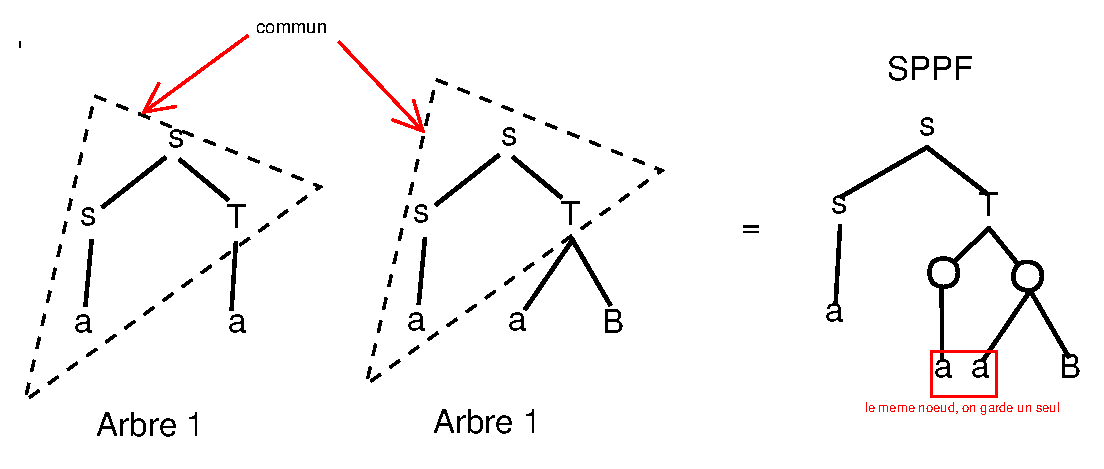
\includegraphics[width=10cm]{Diagramme2.eps}

\section{Earley Alogirithme}
Prenons cette grammaire:
\begin{lstlisting}
S = S + P
| P
P = P * F
| F
F = ( S )
| n
\end{lstlisting}

on veux reconnaitre l'entrée

\begin{tabular}{|l|l|l|l|l|l|l|}
	\hline
	n & + & ( & n & * & n & ) \\ \hline
\end{tabular}

A l'étape 0, le calcule démarre avec l'ensemble E(0) et les règles de l'axiome 'S'


\begin{tabular}{|c|}
	\hline
	\textbf{E(0)}                                                       \\ \hline
	\begin{tabular}[c]{@{}c@{}}S = •S + P (0)\\ S = •P (0)\end{tabular} \\ \hline
\end{tabular}

la prédiction du premier item de E(0) nous donnera les mêmes 2 items de E(0), et donc pas besoin de faire quoi que se sois, donc une la grammaire récursive gauche ne posera pas de problème a notre algorithme.

La prédiction du deuxième item de E(0) générera deux nouveaux items:

\begin{tabular}{|c|}
	\hline
	\textbf{E(0)}                                                                                    \\ \hline
	\begin{tabular}[c]{@{}c@{}}S = •S + P (0)\\ S = •P (0)\\ P = •P * F (0)\\ P = •F (0)\end{tabular} \\ \hline
\end{tabular}

Le prédiction du 3ème item de E(0) ne sert a rien. La prédiction du 4ème item de E(0) générera deux nouveaux items supplémentaire:

\begin{tabular}{|c|}
	\hline
	\textbf{E(0)}                                                                                                                   \\ \hline
	\begin{tabular}[c]{@{}c@{}}S = •S + P (0)\\ S = •P (0)\\ P = •P * F (0)\\ P = •F (0)\\ F = •( S ) (0)\\ F = •n (0)\end{tabular} \\ \hline
\end{tabular}

La Lecture du 5ème item de E(0) échoue puisque le symbole ne correspond pas a l'entrée.

La lecture du 6ème item se fait avec succès, est génère un nouveau item dans l'ensemble suivant E(1)

\begin{tabular}{|c|}
	\hline
	\textbf{E(1)} \\ \hline
	F = n• (0)    \\ \hline
\end{tabular}

On a traité tout les items de E(0), attaquons nous a l'ensemble E(1)

La Complétion du premier item de E(1), nous fait ajouter le 4ème item de E(0) a E(1):

\begin{tabular}{|c|}
	\hline
	\textbf{E(1)}                                                   \\ \hline
	\begin{tabular}[c]{@{}c@{}}F = n• (0)\\ P = F• (0)\end{tabular} \\ \hline
\end{tabular}

la Complétion du deuxième item de E(1), nous fait ajouter le deuxième et troisième item de E(0) dans E(1)

\begin{tabular}{|c|}
	\hline
	\textbf{E(1)}                                                                                 \\ \hline
	\begin{tabular}[c]{@{}c@{}}F = n• (0)\\ P = F• (0)\\ S = P• (0)\\ P = P• * F (0)\end{tabular} \\ \hline
\end{tabular}

...

Au finale notre table Earley ressemblera a :

\begin{tabular}{lllllllll}
	\cline{1-1} \cline{3-3} \cline{5-5} \cline{7-7} \cline{9-9}
	\multicolumn{1}{|c|}{\textbf{E(0)}}                                                                                                                   & \multicolumn{1}{c|}{\textbf{}} & \multicolumn{1}{c|}{\textbf{E(1)}}                                                                                                                       & \multicolumn{1}{c|}{}          & \multicolumn{1}{c|}{\textbf{E(2)}}                                                                                                      & \multicolumn{1}{l|}{} & \multicolumn{1}{c|}{\textbf{E(3)}}                                                                                                                                    & \multicolumn{1}{c|}{\textbf{}} & \multicolumn{1}{c|}{\textbf{E(4)}}                                                                                                                   \\ \cline{1-1} \cline{3-3} \cline{5-5} \cline{7-7} \cline{9-9} 
	\multicolumn{1}{|l|}{\begin{tabular}[c]{@{}l@{}}S = •S + P (0)\\ S = •P (0)\\ P = •P * F (0)\\ P = •F (0)\\ F = •( S ) (0)\\ F = •n (0)\end{tabular}} & \multicolumn{1}{l|}{}          & \multicolumn{1}{l|}{\begin{tabular}[c]{@{}l@{}}F = n• (0)\\ P = F• (0)\\ S = P• (0)\\ P = P• * F (0)\\ S = S• + P (0)\end{tabular}}                      & \multicolumn{1}{l|}{}          & \multicolumn{1}{l|}{\begin{tabular}[c]{@{}l@{}}S = S + •P (0)\\ P = •P * F (2)\\ P = •F (2)\\ F = •( S ) (2)\\ F = •n (2)\end{tabular}} & \multicolumn{1}{l|}{} & \multicolumn{1}{l|}{\begin{tabular}[c]{@{}l@{}}F = ( •S ) (2)\\ S = •S + P (3)\\ S = •P (3)\\ P = •P * F (3)\\ P = •F (3)\\ F = •( S ) (3)\\ F = •n (3)\end{tabular}} & \multicolumn{1}{l|}{}          & \multicolumn{1}{l|}{\begin{tabular}[c]{@{}l@{}}F = n• (3)\\ P = F• (3)\\ S = P• (3)\\ P = P• * F (3)\\ S = S• + P (3)\\ F = ( S• ) (2)\end{tabular}} \\ \cline{1-1} \cline{3-3} \cline{5-5} \cline{7-7} \cline{9-9} 
	&                                &                                                                                                                                                          &                                &                                                                                                                                         &                       &                                                                                                                                                                       &                                &                                                                                                                                                      \\ \cline{1-1} \cline{3-3} \cline{5-5}
	\multicolumn{1}{|c|}{\textbf{E(5)}}                                                                                                                   & \multicolumn{1}{c|}{\textbf{}} & \multicolumn{1}{c|}{\textbf{E(6)}}                                                                                                                       & \multicolumn{1}{c|}{\textbf{}} & \multicolumn{1}{c|}{\textbf{E(7)}}                                                                                                      &                       &                                                                                                                                                                       &                                &                                                                                                                                                      \\ \cline{1-1} \cline{3-3} \cline{5-5}
	\multicolumn{1}{|l|}{\begin{tabular}[c]{@{}l@{}}P = P * •F (3)\\ F = •( S ) (5)\\ F = •n (5)\end{tabular}}                                            & \multicolumn{1}{l|}{}          & \multicolumn{1}{l|}{\begin{tabular}[c]{@{}l@{}}F = n• (5)\\ P = P * F• (3)\\ S = P• (3)\\ P = P• * F (3)\\ F = ( S• ) (2)\\ S = S• + P (3)\end{tabular}} & \multicolumn{1}{l|}{}          & \multicolumn{1}{l|}{{\color[HTML]{333333} \begin{tabular}[c]{@{}l@{}}F = ( S )• (2)\\ P = F• (2)\\ S = S + P• (0)\end{tabular}}}        &                       &                                                                                                                                                                       &                                &                                                                                                                                                      \\ \cline{1-1} \cline{3-3} \cline{5-5}
\end{tabular}

Le mot est reconnu uniquement si on a un item de la forme (S = $\alpha$ • (0)) dans E(7), ce qui est le cas dans notre exemple.

\section{Essayant de construire un l'Analyseur Earley}
Earley lui même a donné un brève description sur comment construire une représentation de tout les dérivations possible a partir de l'algorithme de base qui ne fais que de la reconnaissance. Et il dit aussi que sa ne requière qu'une complexité cubique en temps et en mémoire au pire des cas.

L'idée de Earley est très simple, a chaque fois qu'on fait une complétion, on ajoute un pointeur depuis chaque symbole non terminale a gauche du point du nouveau item, vers les items qui ont engendrés cette item.

Prenons cette grammaire:
\begin{lstlisting}
S = S T 
  | a ;
B = ;
T = a B 
  | a ;
\end{lstlisting}
On applique l'idée d'Earley précédente pour reconnaitre le mot \lstinline|aa|, on aura:

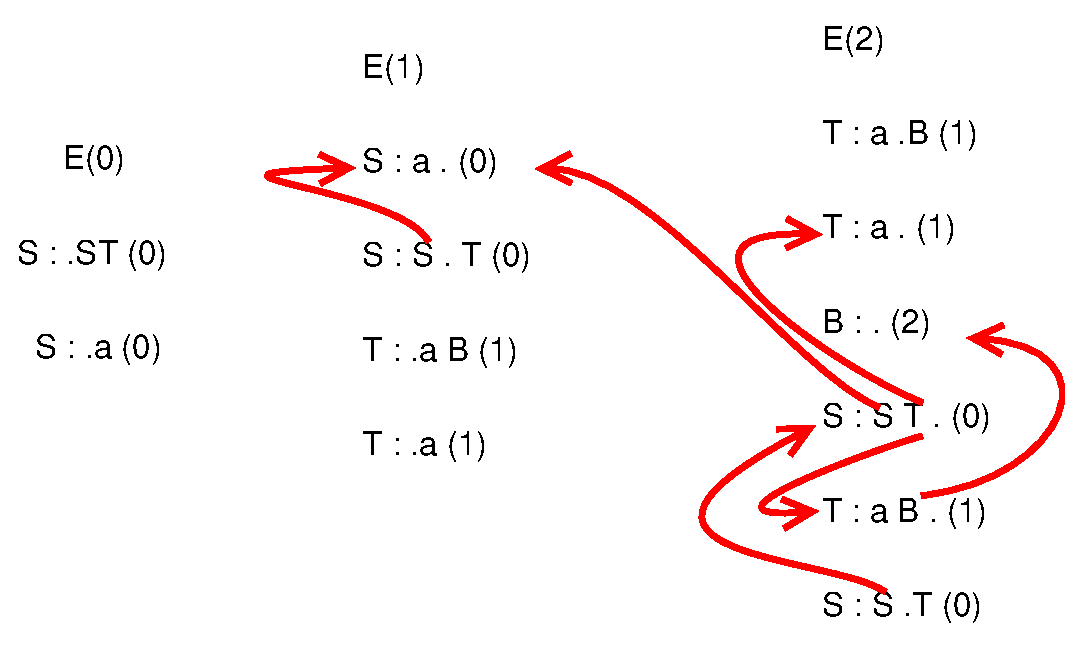
\includegraphics[width=8cm]{Diagramme1.eps}

Ce qui se traduira par la représentation SPPF suivante:

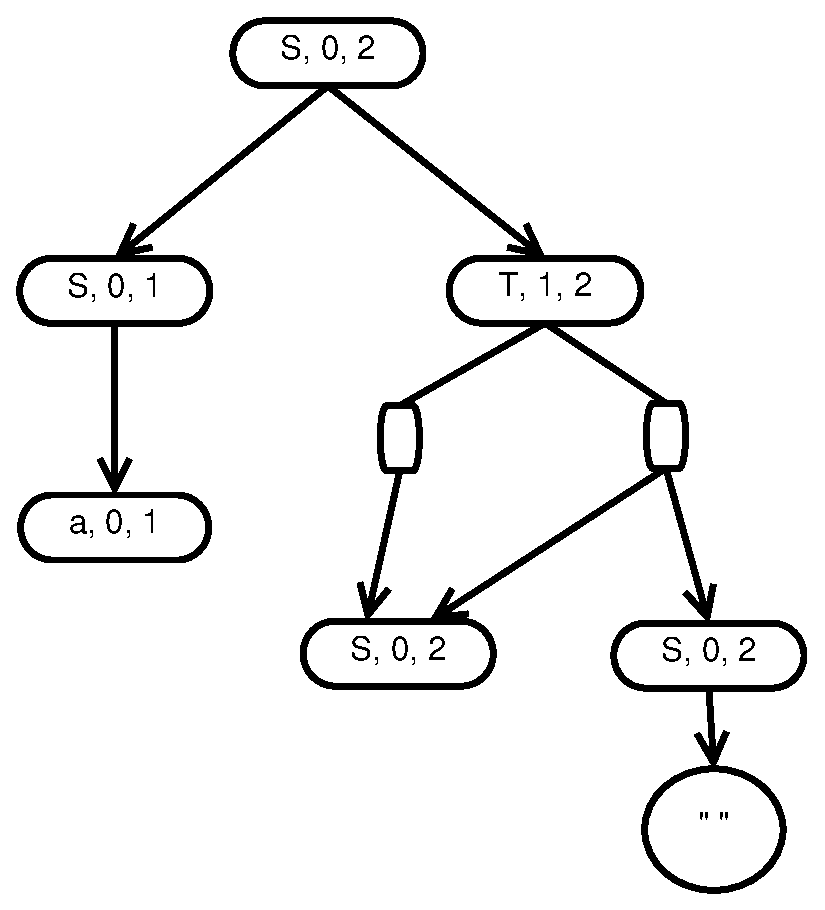
\includegraphics[width=6cm]{Diagramme3.eps}

On vois bien que cette représentation inclue bien tout les dérivations possible du mot \lstinline|aa|, on va pouvoir se dire qu'on a trouver notre algorithme d'analyse syntaxique basé sur Earley, malheureusement, dans certain cas, cette modification de l'algorithme d'Earley pour le transformer en analyseur syntaxique, n'ai pas suffisant. 

Prenons un autre exemple pour démontrer sa:
\begin{lstlisting}
S = SSS 
  | SS
  | b;
\end{lstlisting}

On appliquant la modification d'Earley sur le mot \lstinline|bbb| on aura le SPPF suivant:

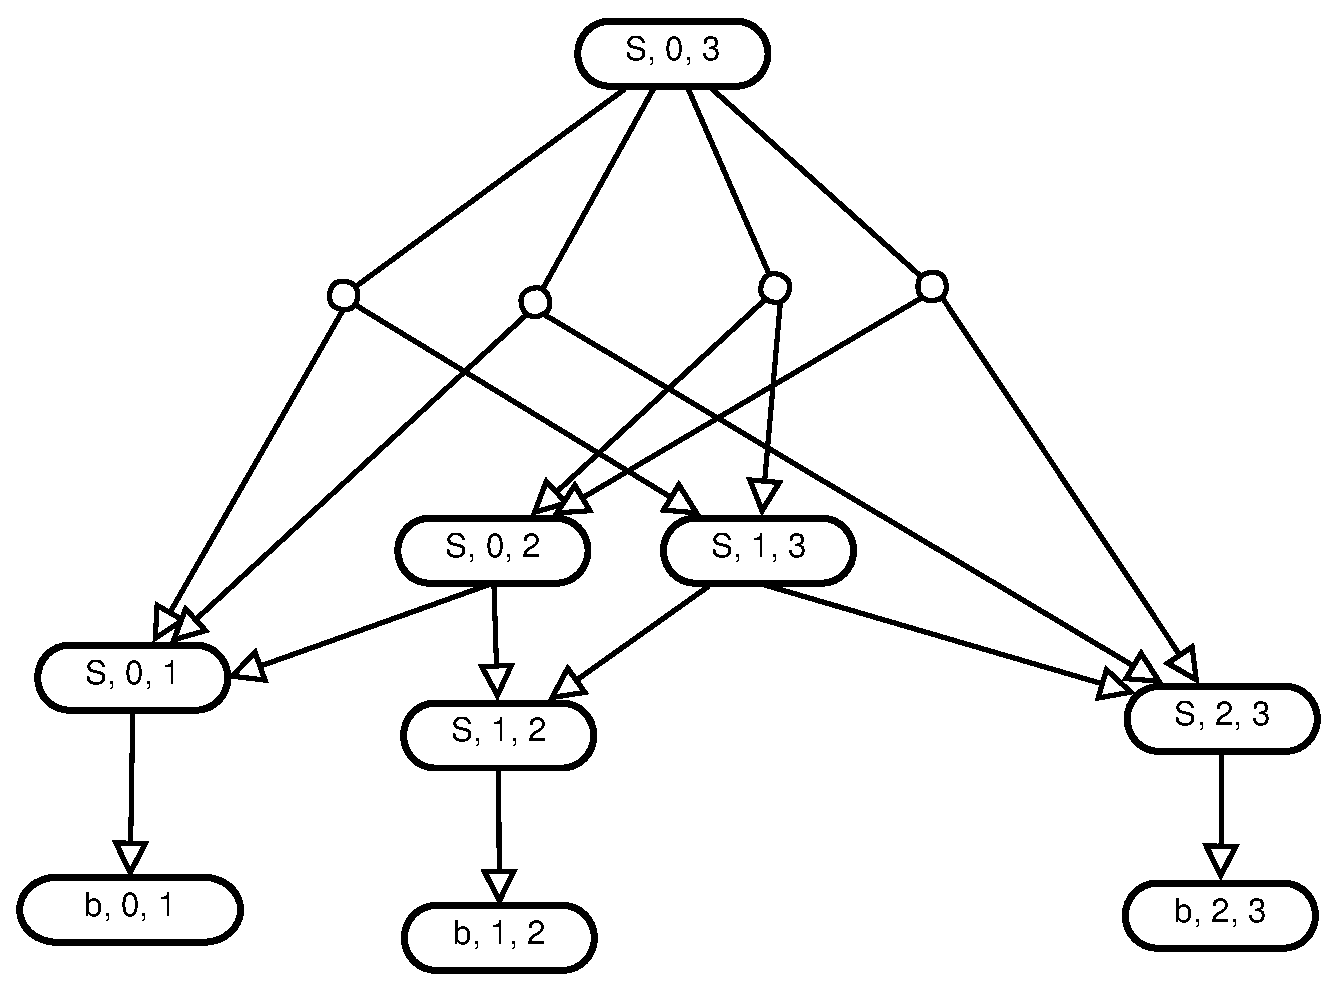
\includegraphics[width=6cm]{Diagramme4.eps}

Cette représentation SPPF contient des dérivations superflus qui sert a reconnaitre les mot \lstinline|bb| et \lstinline|bbbb|, alors que nous voulions juste connaitre les dérivations du mot \lstinline|bbb|. Dans la page 74\cite{Tomita}, Tomita nous explique qu'ajouter plusieurs pointeurs a la même instance du symbole non terminale est une mauvaise idée et résulte sur des dérivation superflus d'autre mot.

Il existe une solution très simple a ce problème. il suffit de dupliquer la règle qui cause se problème. Dans l'exemple précédent, on aura deux règles "S = SS • (0)" identique dans E(3) mais avec des pointeurs différents, ce qui engendrera cette représentation SPPF:

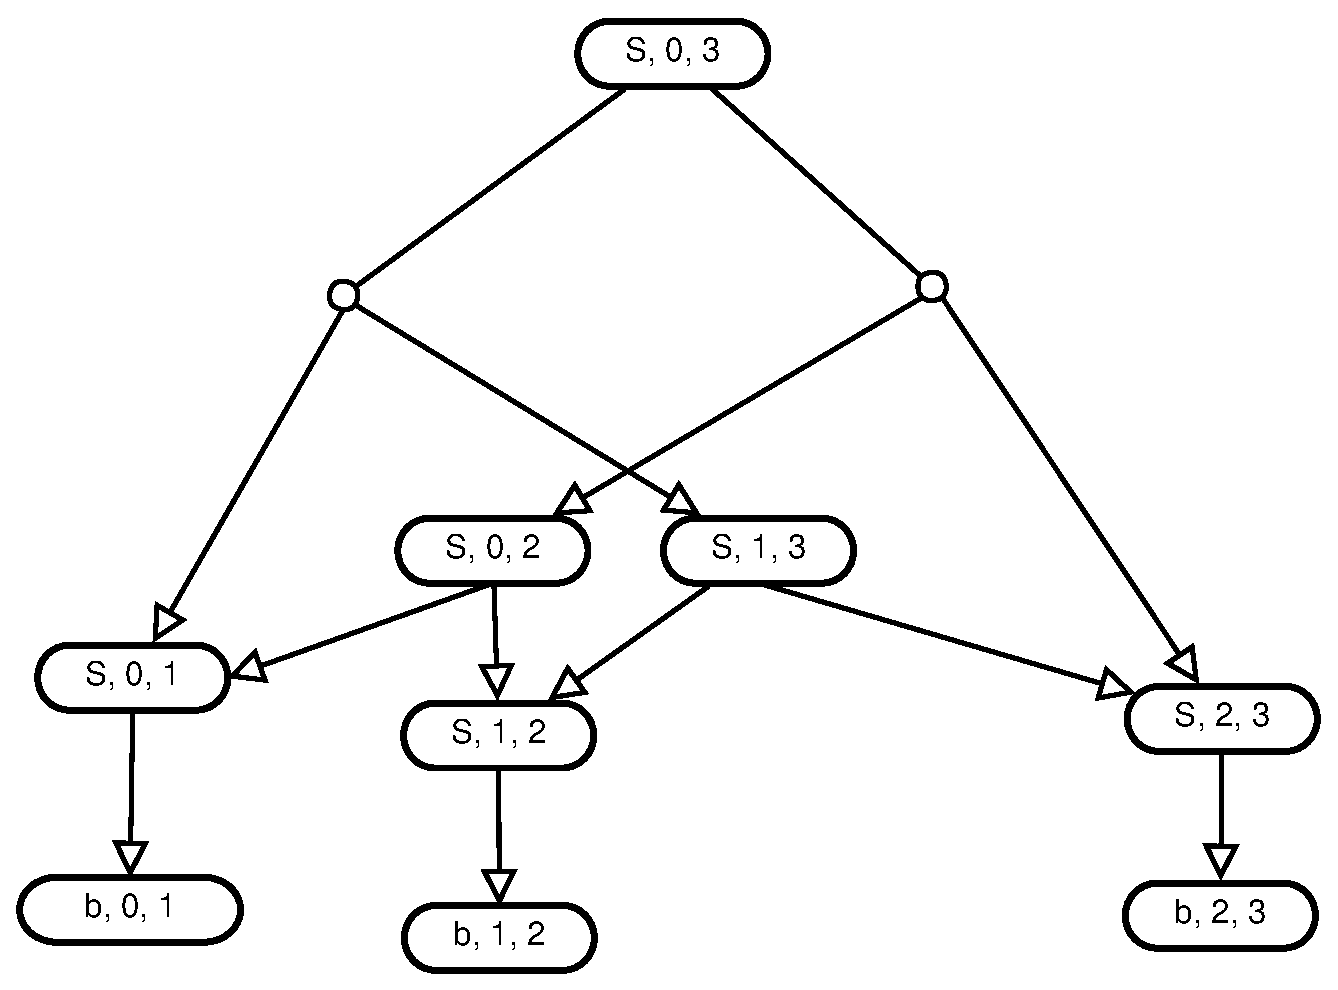
\includegraphics[width=6cm]{Diagramme5.eps}

cette fois si c'est la bonne, la duplication de la règle problématique a permis d'exclure les dérivations superflu.

On viens de trouver un algorithme d'analyse syntaxique basé sur Earley, mais quand est-il de la complexité ? Ben, comme démontrer par Johnson\cite{Johnson} pour un problème similaire et comme confirmé par Scott\cite{Scott}, la complexité polynomiale est infinie. On peut se dire qu'on a gardé l'algorithme de base d'Earley et donc la complexité aurais du être $O(n^3)$, mais la duplication des règles engendrent un problème, en effet, la taille de la table d'Earley ne peut être borné par $O(n^p)$ pour n'importe quelle entier p. Et puisque la complexité en taille et en temps sont liées, on aura une complexité polynomiale infinie.

\chapter{Introduction}
\section{Qu'est ce que l'alogirthme Earley ?}
L'algorithme Earley\footnote{text}, est un, parmi les nombreux algorithmes d'analyse syntaxique, est comme tout ces algorithmes, \textbf{Earley} a besoin d'une grammaire
\begin{lstlisting}
S = S + P
  | P
P = P * F
  | F
F = ( S )
  | n

\end{lstlisting}
... pour transformer une chaine de mot ...

\begin{tabular}{|l|l|l|l|l|l|l|l|l|}
	\hline
	n & + & ( & n & * & n & + & n & ) \\ \hline
\end{tabular}

... en un jolie arbre syntaxique (AST)

\begin{tikzpicture}[sibling distance=5em,
every node/.style = {shape=rectangle, rounded corners,
	draw, align=center,
	top color=white, bottom color=blue!20}]]

\node {S}
child { node {S} 
        child { node {n} } }
child { node {+} }
child { node {P}
	child { node {F}
			child { node {(}}
			child { node {...}}
			child { node {)} } } };
\end{tikzpicture}

Jusqu'à présent rien de spéciale comparé au autre algotithme qu'on conné. 
\section{Pourquoi devrions-nous nous soucier?}
Le plus grand avantage d'Erley, est sans doute son accessibilité. La plus part des autres algorithme offre une restriction sur le type de grammaires, utilisé une grammaire récursif gauche et en rentrera dans une boucle infini, utilisé un autre type et l'algorthme ne marchera plus. Biensur il y a des counternement qu'on peux faire, mais souvant sa complique d'avantage l'algorithme et rendra le travaille plus complexe.

Pour dire simple Earley marche avec tout.

D'une autre part, pour avoir cette généralité, nous devons sacrifié la vitesse. On ne pourra donc pas rivaliser avec des algorithme comme Flex/Bison en terme de rapidité brute. Ce n'ai si grave, puisque
\begin{itemize}
	\item Earley a une complixité cubique O(3), dans les pires des cas, ces meme cas qui ne pourons etre trété pas d'autre algorithme
	\item La plus part des grammaire simple aurons une complexité linaire
	\item Meme la pire grammaire nom-ambigue pourra etre analyser en O(3)
\end{itemize}
\section{Vocabulaire}
Du point de vu de l'algorithme Earley, la grammaire est constitué de règle. Voici un exemple de règle
\begin{lstlisting}
S = S + P
\end{lstlisting}
S est un symbole non terminale, et tout ce qui ne commence pas avec une lettre majuscule est considéré comme étant un symbole terminale (le symbole + dans notre exemple).

Dans le jargons d'Earley, il y a la notion d'items, Voici un item:
\begin{lstlisting}
A = B • * C  (4)
\end{lstlisting}
c'est juste une règles de grammaire avec des informations en plus, qui représente une reconnaissance partielle.
\begin{itemize}
	\item Le point représente la position courante qui indique jusq'ou on a parvenu a parser
	\item Le chiffre 4 représente la position initial sur l'entré qu'on veux parser
\end{itemize}

De plus Earley introduit la notion d'ensemble d'items, chaque ensemble est carterisé par le fait que les item qui y sont associé, ont la même position courante

Et tout ces ensemble la, sont souvent nommé table Earley

\section{Prédiction, Lecture et Complétion}

Pour construire la table Earley, on a besoin de définir trois opérations élémentaire qui s'applique sur un item pour produire un autre item:
\begin{itemize}
	\item Prédiction: le symbole a droite du point est un nom terminal, on ajoute les réglés de ce symbole au même ensemble 
	\item Lecture: le symbole a droite du point est un terminal, on regarde si se symbole coïncide avec la position courante, si oui, on ajoute cette item a l'ensemble suivant.
	\item Complétion: in n'ya rien a droite du point, et dans se cas il ya reconnaissance partielle, on regarde l'item parent, et on l'ajoute a cette ensemble
\end{itemize}

\section{Exemple de construction de table d'Earley}
Reprenons cette grammaire:
\begin{lstlisting}
S = S + P
| P
P = P * F
| F
F = ( S )
| n
\end{lstlisting}

on veux reconnaitre l'entrée

\begin{tabular}{|l|l|l|l|l|l|l|}
	\hline
	n & + & ( & n & * & n & ) \\ \hline
\end{tabular}

A l'étape 0, le calcule démarre avec l'ensemble E(0) et les règles de l'axiome 'S'


\begin{tabular}{|c|}
	\hline
	\textbf{E(0)}                                                       \\ \hline
	\begin{tabular}[c]{@{}c@{}}S = •S + P (0)\\ S = •P (0)\end{tabular} \\ \hline
\end{tabular}

la prédiction du premier item de E(0) nous donnera les mêmes 2 items de E(0), et donc pas besoin de faire quoi que se sois, donc une la grammaire récursive gauche ne posera pas de problème a notre algorithme.

La prédiction du deuxième item de E(0) générera deux nouveaux items:

\begin{tabular}{|c|}
	\hline
	\textbf{E(0)}                                                                                    \\ \hline
	\begin{tabular}[c]{@{}c@{}}S = •S + P (0)\\ S = •P (0)\\ P = •P * F (0)\\ P = •F (0)\end{tabular} \\ \hline
\end{tabular}

Le prédiction du 3ème item de E(0) ne sert a rien. La prédiction du 4ème item de E(0) générera deux nouveaux items supplémentaire:

\begin{tabular}{|c|}
	\hline
	\textbf{E(0)}                                                                                                                   \\ \hline
	\begin{tabular}[c]{@{}c@{}}S = •S + P (0)\\ S = •P (0)\\ P = •P * F (0)\\ P = •F (0)\\ F = •( S ) (0)\\ F = •n (0)\end{tabular} \\ \hline
\end{tabular}

La Lecture du 5ème item de E(0) échoue puisque le symbole ne correspond pas a l'entrée.

La lecture du 6ème item se fait avec succès, est génère un nouveau item dans l'ensemble suivant E(1)

\begin{tabular}{|c|}
	\hline
	\textbf{E(1)} \\ \hline
	F = n• (0)    \\ \hline
\end{tabular}

On a traité tout les items de E(0), attaquons nous a l'ensemble E(1)

La Complétion du premier item de E(1), nous fait ajouter le 4ème item de E(0) a E(1):

\begin{tabular}{|c|}
	\hline
	\textbf{E(1)}                                                   \\ \hline
	\begin{tabular}[c]{@{}c@{}}F = n• (0)\\ P = F• (0)\end{tabular} \\ \hline
\end{tabular}

la Complétion du deuxième item de E(1), nous fait ajouter le deuxième et troisième item de E(0) dans E(1)

\begin{tabular}{|c|}
	\hline
	\textbf{E(1)}                                                                                 \\ \hline
	\begin{tabular}[c]{@{}c@{}}F = n• (0)\\ P = F• (0)\\ S = P• (0)\\ P = P• * F (0)\end{tabular} \\ \hline
\end{tabular}

...

Au finale notre table Earley ressemblera a :

\begin{tabular}{lllllllll}
	\cline{1-1} \cline{3-3} \cline{5-5} \cline{7-7} \cline{9-9}
	\multicolumn{1}{|c|}{\textbf{E(0)}}                                                                                                                   & \multicolumn{1}{c|}{\textbf{}} & \multicolumn{1}{c|}{\textbf{E(1)}}                                                                                                                       & \multicolumn{1}{c|}{}          & \multicolumn{1}{c|}{\textbf{E(2)}}                                                                                                      & \multicolumn{1}{l|}{} & \multicolumn{1}{c|}{\textbf{E(3)}}                                                                                                                                    & \multicolumn{1}{c|}{\textbf{}} & \multicolumn{1}{c|}{\textbf{E(4)}}                                                                                                                   \\ \cline{1-1} \cline{3-3} \cline{5-5} \cline{7-7} \cline{9-9} 
	\multicolumn{1}{|l|}{\begin{tabular}[c]{@{}l@{}}S = •S + P (0)\\ S = •P (0)\\ P = •P * F (0)\\ P = •F (0)\\ F = •( S ) (0)\\ F = •n (0)\end{tabular}} & \multicolumn{1}{l|}{}          & \multicolumn{1}{l|}{\begin{tabular}[c]{@{}l@{}}F = n• (0)\\ P = F• (0)\\ S = P• (0)\\ P = P• * F (0)\\ S = S• + P (0)\end{tabular}}                      & \multicolumn{1}{l|}{}          & \multicolumn{1}{l|}{\begin{tabular}[c]{@{}l@{}}S = S + •P (0)\\ P = •P * F (2)\\ P = •F (2)\\ F = •( S ) (2)\\ F = •n (2)\end{tabular}} & \multicolumn{1}{l|}{} & \multicolumn{1}{l|}{\begin{tabular}[c]{@{}l@{}}F = ( •S ) (2)\\ S = •S + P (3)\\ S = •P (3)\\ P = •P * F (3)\\ P = •F (3)\\ F = •( S ) (3)\\ F = •n (3)\end{tabular}} & \multicolumn{1}{l|}{}          & \multicolumn{1}{l|}{\begin{tabular}[c]{@{}l@{}}F = n• (3)\\ P = F• (3)\\ S = P• (3)\\ P = P• * F (3)\\ S = S• + P (3)\\ F = ( S• ) (2)\end{tabular}} \\ \cline{1-1} \cline{3-3} \cline{5-5} \cline{7-7} \cline{9-9} 
	&                                &                                                                                                                                                          &                                &                                                                                                                                         &                       &                                                                                                                                                                       &                                &                                                                                                                                                      \\ \cline{1-1} \cline{3-3} \cline{5-5}
	\multicolumn{1}{|c|}{\textbf{E(5)}}                                                                                                                   & \multicolumn{1}{c|}{\textbf{}} & \multicolumn{1}{c|}{\textbf{E(6)}}                                                                                                                       & \multicolumn{1}{c|}{\textbf{}} & \multicolumn{1}{c|}{\textbf{E(7)}}                                                                                                      &                       &                                                                                                                                                                       &                                &                                                                                                                                                      \\ \cline{1-1} \cline{3-3} \cline{5-5}
	\multicolumn{1}{|l|}{\begin{tabular}[c]{@{}l@{}}P = P * •F (3)\\ F = •( S ) (5)\\ F = •n (5)\end{tabular}}                                            & \multicolumn{1}{l|}{}          & \multicolumn{1}{l|}{\begin{tabular}[c]{@{}l@{}}F = n• (5)\\ P = P * F• (3)\\ S = P• (3)\\ P = P• * F (3)\\ F = ( S• ) (2)\\ S = S• + P (3)\end{tabular}} & \multicolumn{1}{l|}{}          & \multicolumn{1}{l|}{{\color[HTML]{333333} \begin{tabular}[c]{@{}l@{}}F = ( S )• (2)\\ P = F• (2)\\ S = S + P• (0)\end{tabular}}}        &                       &                                                                                                                                                                       &                                &                                                                                                                                                      \\ \cline{1-1} \cline{3-3} \cline{5-5}
\end{tabular}

On arrive donc a la fin (TODO : condition de reussite)
\section{Que va t'on faire ?}
Nous allons crée un programme qui va avoir en entré une grammaire, est aura en sorti un analyseur syntaxique suivant l'algorithme Earley.

Par la suite en va modifier cette algorithme pour notre besoin (TO DO :)

\chapter{Développement de l'outils}
Le programme sera écrit en C++, mais sera facilement traduit dans d'autre langage si nécessaire.
\section{Petite Pré-analyse avant de commencer}
Notre outils aura en entrée une grammaire est en sortie, on aura un analyseur syntaxique. Plusieurs question se sont posés durant le développement de cette outils, Voila un récapitulatif des décision prise:
\begin{itemize}
	\item Nous appellerons notre programme earley
	\item La première entrée de notre programme, sera un fichier, qui contiendra la description de la grammaire en format Yacc
	\item La deuxième entrée de notre programme sera un deuxieme fichier, qui contiendra la chaine a analyser.
	\item La sorti sera un troisième fichier contenant L'AST
	\item Les noms de varibale, et de fonction serons en anglais, referai vous donc au dictionnaire (a faire)
\end{itemize}

Le programme sera exécuter en ligne de commande suivant la syntaxe suivant: 

earley <file1> <file2> <file3>

file1 : le fichier de grammaire
file2 : le fichier contenant la chaine a analysé
file3 : le fichier contenant l'AST

\section{Le Format Yacc}
Pour la grammaire que nous fournissons au programme, nous utiliserons le format Yacc simplifié suivant:

Une règle de grammaire a la forme:

A  :  BODY  ;

A représente un symbole non-terminal, et BODY représente une séquence de zéro ou plus de terminaux et non-terminaux. La côlon et le point-virgule sont la ponctuation de Yacc.

un symbole terminal doit être déclaré comme telle au debut du fichier:

\%token  n1  n2  p

Si un symbole non terminal correspond à la chaîne vide, cela peut être indiqué de manière évidente:

A : ;

le symbole de départ est considéré comme le côté gauche de la première règle de grammaire dans la section des règles
\bibliographystyle {plain}
\bibliography{mabiblio}             
\end{document}